\chapter{Architecture and Design of the WPT System} \label{C:architecture}
Once the inductive coupling system has been studied in detail, it is time to outfit the selected coil model C on the drone. The selection of this model is argued in Chapter \ref{C:experimental}, after all the measures are performed. In this chapter, the required circuits to design the WPT system are discussed. In the first section, the nano-quadcopter used is introduced and all its main features are explained, as well as the necessity of designing brand new motor mounts in order to support the coil. 

In the second part of the chapter, the architecture of the transmitter and receiver circuits is explained, as well as its design. The main feature of the WPT system lies on energy conversion. Hence, both the transmitter and the receiver circuits need of power converters. As shown in Figure \ref{F:blockDiagram} the transmitter includes a ultra low DC-DC converter and a DC-AC converter. At the receiving side, the power converters include at least an AC-DC converter. Later, for the used application, a DC-DC converter will be introduced for the battery recharging circuit.

%%%
%%%
%%% SE ESCOGE LA BOBINA C !!! EXPLICAR QUE TODO EL CAPITULO SE TIENE EN CUENTA
%%%
%%%

\begin{figure}[htb]
\begin{center}
\vspace{+0.5em}
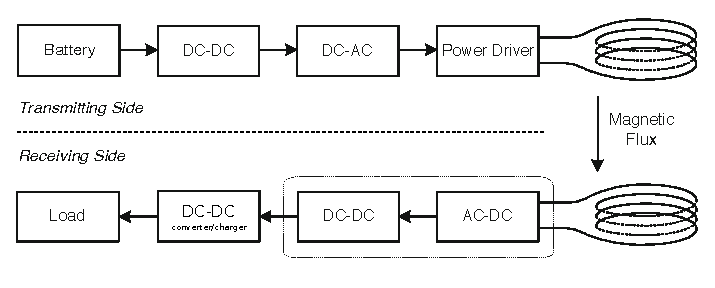
\includegraphics[width=0.9\textwidth]{./images/block2}
% \vspace{-1.5em}
\caption{Block diagram}
\label{F:blockDiagram}
\end{center}
\end{figure}


  \section{Quadcopter}
One of the initial objectives of the project is the WPT system outfitting on the nano-quadcopter. The inclusion of the quadcopter as an energy \textit{transporter} restricts both transmitter and receiver side, but mainly the transmitter because of the weight. The model used in this work is the created by \textit{Bitcraze}, its second nano-quadcopter version, named \textit{Crazyflie 2.0}. 

The assembly of this quadcopter can be divided into two parts. The first is composed by the battery, motors and headers attaching. In the second, the propellers are introduced and balanced. This last procedure is really important due the fact that well balanced propellers reduce vibrations in the copter and noise in the sensors improving the stability of the \textit{Crazyflie}.


\begin{figure}[H]
\centering
\begin{subfigmatrix}{2}
\vspace{1em} 
\hspace*{\fill}%
\subfigure[Crazyflie 2.0] 
  {\includegraphics[width=2.2in]{./images/crazyflie}}\hfill 
\subfigure[CrazyRadio USB dongle]
  {\includegraphics[width=2.0in]{./images/CrazyRadio}}
\hspace*{\fill}%
\end{subfigmatrix}
\caption{Transmitter circuit}
% \label{F:transmitter}
\end{figure}

Contrary to other drones, \textit{Crazyflie} allowed us the possibility to fly it indoor. It also has many interesting features listed in Table \ref{F:crazyflieFeatures} which made us to select it. Owing to the fact that \textit{Crazyflie} is an open source project it is possible to log, graph and set variables in real-time via the USB radio dongle.

\begin{figure}[htb]
\begin{center}
\begin{tabular}{|c|c|}

  \hline
  \multicolumn{2}{|c|}{\bf{Crazyflie 2.0 specification}} \\
  \hline
  \hline
  Size (WxHxD)  & 92x92x29 mm \\ \hline
  \multirow{2}{*}{Radio specs} 
   &  Low energy Bluetooth\\
   &  Radio amplifier 1 km range \\ \hline
  \multirow{3}{*}{Controllers} 
   &  STM32F405 MCU\\
   &  $\mu$USB connector \\
   &  USB OTG capability \\ \hline
  \multirow{3}{*}{IMU} 
   &  3 axis gyro \\
   &  3 axis accelerometer \\
   &  3 axis magnetometer \\
   &  Pressure sensor \\
  \hline

\end{tabular}
\caption{Crazyflie 2.0 features}
\label{F:crazyflieFeatures}
\end{center}
\end{figure}


    \subsection{Controlling the \textit{Crazyflie}}
As it is shown in Table \ref{F:crazyflieFeatures}, the \textit{Crazyflie} can be either controlled by a mobile device or a computer. Using a mobile device is the fastest way to control it, but its maneuverability is reduced compared to the computer option. Therefore, this last one is chosen.

The two needed requirements for flying the \textit{Crazyflie} using a computer are: a radio USB dongle (\textit{Crazyflie PA}) for communication and a standard gamepad for maneuvering. In addition, a virtualization program is required to run the \textit{Crazyflie} client. Few drivers are needed, as well as the last updated software in order to avoid any \textit{bug}. Both drivers and the needed code are uploaded on \textit{GitHub} repositories \cite{github}. 

\begin{figure}[H]
\centering
\includegraphics[width=0.65\textwidth]{./images/virtual}
\caption{Crazyflie's computer client}
\end{figure}


  \subsection{Motor Mount Design}

With the original design of the \textit{Crazyflie} nano-quadcopter is almost impossible to install it the used coil. As a consequence, in this case, the coil would not be subjected neither precisely, nor ``smartly''. The solution is to redesign the motor mounts of the \textit{Crazyflie} to accomplish a good coil support.

Using the CAD software \textit{SolidWorks}, it has been designed a motor mount with the same characteristics of the original mounts. The only difference is that the designed structure is made to place the coil under the \textit{Crazyflie}. 


This structure has the main characteristic of supporting lateral stresses, as the \textit{default} mounts, and also to prevent the fall of the coil, by using a kind of hook placed at the end of the mount arm. The complete design schematics are located in the Appendices. All this mentioned characteristics are showed in Figures \ref{F:MM} and \ref{F:MMC}. 

\begin{figure}[H]
\centering
\begin{subfigmatrix}{3} 
\subfigure[Plan and elevation views] 
  {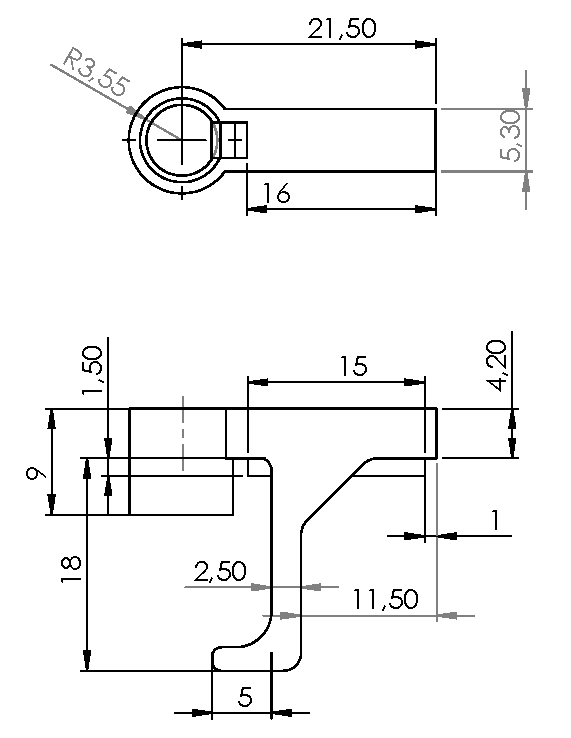
\includegraphics{./images/plantaAlzado}\label{F:MM}}
\subfigure[3D model] 
  {\includegraphics{./images/3dmount}\label{F:MMC}}
\subfigure[Real view image]
  {\includegraphics{./images/FullSizeRender}\label{F:finalMount}}
\end{subfigmatrix}
\caption{Motor mount process design}
\end{figure}

Once the motor mount is designed it can be printed with a 3D printer. The result is exhibited in Figure \ref{F:finalMount}.



  \section{Transmission System}

In a WPT system, the transmitter is intended for carrying power in order to satisfy the receiver demand. Its design is based on two premises; size and weight. Size is important in order to maintain the nano-quadcopter balanced owing to \textit{Crazyflie} is not designed to carry objects. The weight constraint is repeated several times during this project.

% Therefore, weight is the parameter which will define transmission subsystems.

    \subsection{Power Source}
After considering different options, such as using two isolated batteries for feeding the drone and the induction system separately, we decided to use the default battery of the nano-quadcopter, and so avoiding to increase the total weight. The battery \textit{Crazyflie} uses is of the type LiPo (Lithium-Polymer).
    
\begin{figure}[htb]
\begin{center}
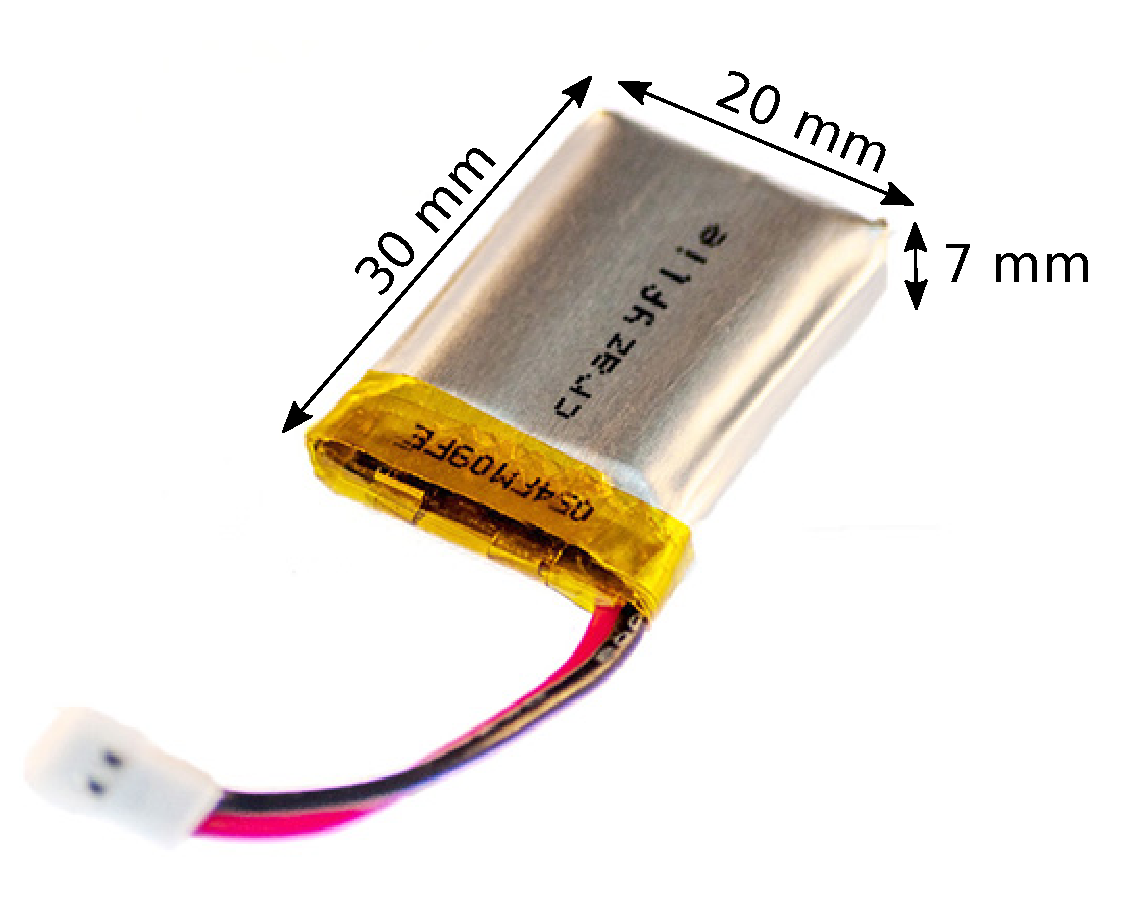
\includegraphics[width=0.4\textwidth]{./images/battery}
\caption{Crazyflie's battery size}
\label{F:battery}
\end{center}
\end{figure}

Althought LiPo is not the safest chemistry, these batteries are currently the most popular type for radiocontrol use. The reason is due to LiPo batteries has the best power to weight ratios and discharge currents. It also allows to use only a single cell.


\begin{table}[ht]
\begin{center}
\begin{tabular}{|c|c|c|c|}

\noalign{\global\arrayrulewidth1pt}
\hline
\textbf{Capacity}  &   \textbf{Nominal voltage}   &   \textbf{Discharge}    &   \textbf{Charge}\\
\hline
\hline
240 mAh   & 3.7 V   &   15C   &   2C  \\ \hline 

\end{tabular}
\caption{Battery's electrical specifications}
\label{T:batterySpecs}
\end{center}
\end{table}

The electrochemical batteries have the advantage over other energy storage devices, such as supercapacitors, that their main discharge curve is exponential, meaning that the energy stays high during most of the charge and then drops rapidly as the charge depletes \cite{batteryDischarge}. The \textit{Crazyflie} battery discharge rate or C-rate is of 15C which means 15-times the rated capacity.

As it is stated in \cite{crazyflie}, the maximum flight time with LiPo battery is up to 7 minutes. Theoretically with motors at full power and consuming 3600 mA, the flight is being reduced to 4 minutes. Regrettably, this time will be even reduced by the inclusion of the induction system. 

The end-of-discharge voltage for most LiPo is 3.0 V/cell. At this level, roughly 95 percent of the energy is spent and the voltage would drop rapidly if the discharge were to continue \cite{batteryDischarge}. To protect the battery from over-discharging, which is very sensitive to, the quadcopter comes with a PCM (Protection Circuit Module) that prevents operation beyond a specified end-of-discharge voltage. 










\subsection{Voltage Regulator}
The voltage regulator was the last system implementation. Owing to the necessity of having 12 V, explained in Chapter \ref{C:experimental}, on the transistor collector, a switching voltage regulator is the most appropriate solution. Linear regulators can only step down the input voltage and the possibility of adding a second battery was rejected because of weight. 

Switching regulators are highly efficient and able to boost, buck and invert voltages with ease, but they also have weaknesses. One of them is that they are complex chips and, consequently, it can take a lot of design effort to get a new product working properly. In addition, the level of integration of contemporary switching regulators does not come cheaply and increases the chip size \cite{regulators}.

To solve these issues the \textit{Webench} application is used. This design tool developed by \textit{Texas Instruments} allows to design the voltage regulator that better adjusts to our input and output power requirements. 

\begin{table}[htb]
\begin{center}
\begin{tabular}{|c|c|c|}

\noalign{\global\arrayrulewidth1pt}
\hline
\textbf{Input Voltage}  &   \textbf{Output Voltage}   &   \bf{Output Current}\\
\hline
\hline
3 - 3.7 V       & 12 V   &   0.5 A  \\ \hline 

\end{tabular}
\caption{Regulator requirements}
\label{T:regulator}
\end{center}
\end{table}

\begin{figure}[H]
  \begin{center}
    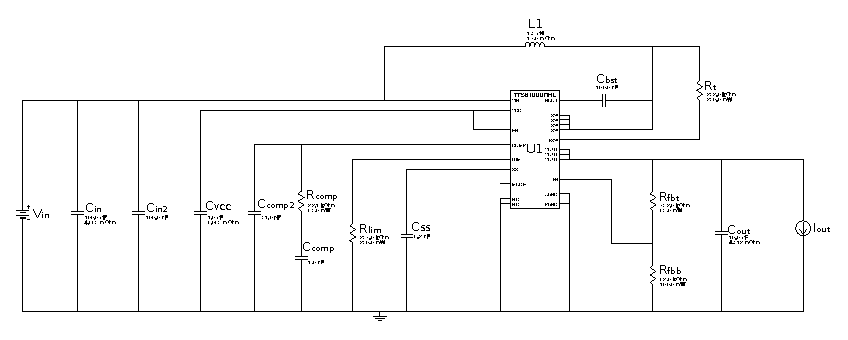
\includegraphics[width=1.05\textwidth]{./images/TPS61088}
  \caption{TPS61088 design circuit}
  \end{center}
\end{figure}

It must be said that the regulator is designed to provide a maximum output current of 500 mA, which is the maximum input current of the power driver, discussed later.

The requirements above lead us to different switching regulators. By looking at size and efficiency, the TPS 61088 was the one with best efficiency per unit of area. The circuit schematic is given in Appendix \ref{Appendix: DC-DC}.

Although an ideal switcher has a $100\%$ efficiency, the actual efficiency is about $92\%$ (Appendix \ref{Appendix: DC-DC}) and it depends on the output current and the input voltage. The power \textit{lost} is really low and it is dissipated following,

\begin{equation}
P_{dis} = \left(\frac{1}{\eta}-1\right)\cdot{P{out}}
\end{equation}


The input current that the regulator is drawing to the battery can be calculated using Equation \ref{eq:regulator}, and it defines the global circuit consumption. 

\begin{equation}\label{eq:regulator}
I_{in} = \left({I_{out}}\cdot\frac{V_{out}}{V_{in}}\right)/{\eta}
\end{equation}

Before computing $I_{in}$, it will be necessary to figure out which is the output current and which relies on the power driver. 









    \subsection{Oscillator} 
A Quartz Crystal Oscillator (XO) is used to generate the necessary periodic signal which generates the alternating current in the \textit{Tx} coil. It is selected for its good performance, a low power consumption, and a simple electronic circuit. This type of oscillator not only provides an extraordinary frequency stability, but it also provides a constant frequency output under varying load conditions, which is an important aspect to consider.

\begin{figure}[H]
\begin{center}
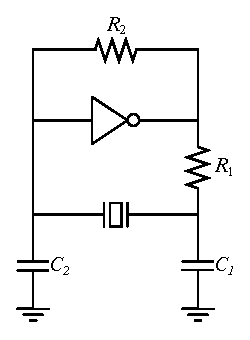
\includegraphics[width=0.3\textwidth]{./images/oscilador}
\caption{Oscillator schematic}
\label{F:oscillator}
\end{center}
\end{figure}

The functioning of the quartz crystal oscillator is based on piezoelectric effect. Piezoelectricity is the primary property of a crystal which makes it usable as resonator. Piezoelectricity is a reversible property of a crystal by which an electrical charge produces a mechanical force by changing the shape of the crystal and vice versa, a mechanical force applied to the crystal produces an electrical charge \cite{quartzCrystal}. 

As it is discussed at the end of the previous chapter, each coil model has its own resonant frequency, and therefore a unique oscillator circuit. For the selected coil model, the resonant frequency is 0.95 MHz. 

The characteristic frequency of the crystal, or rate of vibration, is determined by the cut, size, and shape of the quartz crystal. Therefore, to achieve the desired frequency of 0.95 MHz a special crystal is needed. Hence, taking advantage on the wide Q factor of coils, an standard crystal frequency of 1 MHz is selected. 

\begin{table}[htb]
\begin{center}
\begin{tabular}{|c|c|}

\noalign{\global\arrayrulewidth1pt}
\hline
\textbf{Parameter}  &   \textbf{Value}\\
\hline
\hline
Frequency       & 1 MHz                  \\ \hline 
$R_1$           & 9.1 M$\Omega$          \\ \hline 
$R_2$           & 910 $\Omega$           \\ \hline 
$C_1$           & 47 pF                \\ \hline
$C_2$           & 47 pF                \\ \hline  
Consumption     & 8.4 mA                 \\ \hline

\end{tabular}
\caption{XO parameters}
\label{T:XOparameters}
\end{center}
\end{table}


In figure above, it is represented the Pierce oscillator circuit. This parallel oscillator is a derivative of the Colpitts oscillator. The circuit is implemented using a minimum of components: a single CMOS inverter gate, two resistors, two capacitors and the quartz crystal.

For high speed CMOS logic families, typically \cite{oscilador}:
\begin{itemize}[noitemsep] % To be more compact --> \begin{itemize}[noitemsep,nolistsep]
  \item $R_1$ is between 8.2 M$\Omega$ and 10 M$\Omega$
  \item $R_2$ is between 470 $\Omega$ and 2220 $\Omega$
  \item $C_1$ and $C_2$ are of the order of 62 pF 
\end{itemize}









    \subsection{Power Driver}

The output power delivered from the oscillator is not enough to feed the inductor directly. Thus, a Darlington transistor has been placed after the oscillator to elevate the magnetizing current through the primary coil. This increase in the input power will allow the system to transfer power up to larger distances.

The ULN2803A driver is a high-voltage, high-current Darlington transistor array. The device consists of eight NPN Darlington pairs that feature high-voltage outputs with common-cathode clamp diodes for switching inductive loads. Figure \ref{F:transitor} shows a simplified scheme of the power driver. The complete scheme is attached at Appendix \ref{Appendix: powerDriver}.

\begin{figure}[h]
  \begin{center} 
  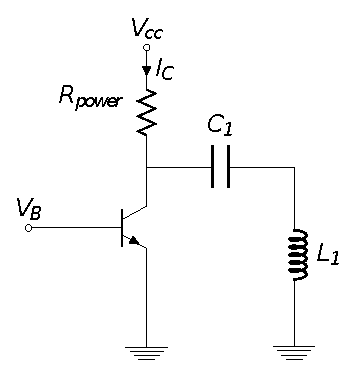
\includegraphics[width=0.4\textwidth]{./images/transistor}
    \caption{Simplified transistor diagram}
    \label{F:transitor}
  \end{center}
\end{figure}

From Figure \ref{F:transitor}, it can be observed that the transistor is working such a switch and driven by the square signal of 0-12 V coming from the oscillator. When an input (pins 1 to 8) is driven ``HIGH'' the corresponding output will switch ``LOW'' sinking current. Likewise, when the input is driven ``LOW'' the corresponding output switches to a high impedance state. This high impedance ``OFF'' state blocks load current and reduces leakage current through the device improving efficiency.

\begin{table}[htb]
\begin{center}
\begin{tabular}{|c|c|}

\noalign{\global\arrayrulewidth1pt}
\hline
\textbf{Parameter}  &   \textbf{Value}\\
\hline
\hline
$V_{CC}$            & 12 V            \\ \hline 
$V_{CE(SAT)}$       & 1.3 V           \\ \hline 
$I_{CC(MAX)}$       & 500 mA          \\ \hline 
$R_{power}$         & 33 $\Omega $      \\ \hline
\end{tabular}
\caption{Electrical characteristics}
\label{T:transistor}
\end{center}
\end{table}


Pin 8 (GND), is connected to the loads ground or 0 volts, while pin 10 ($V_{CC}$) connects to the loads supply. Then any load needs to be connected between +$V_{CC}$ and an output pin, pins 11 to 18. For inductive loads such as coils, pin 10 should always be connected to $V_{CC}$.

The ULN2803A Darlington driver is capable of switching 500 mA per channel. In our case the collector-current $I_{CC}$ is determined using the next expression,

\begin{equation}
I_{CC} = \frac{V_{CC}-V_{CE(SAT)}}{R_{power}}=324\:\textnormal{mA}
\end{equation}

where $R_{power}$ is achieved by combining three resistors in parallel. Each resistor has a resistance value of 100 $\Omega$ and tolerates powers around 1W without any problems. Once the collector current is calculated, it is possible to calculate the total power demanded from the battery. Substituting $I_{CC}$ in equation \ref{eq:regulator} an input current of 1.05 A is obtained. Therefore, the total theoretical power consumed by the transmitter is:

\begin{equation}
P_{in} = V_{in}\cdot{I_{in}}=3.88\:\textnormal{W}
\end{equation} 

It must be also considered the maximum switching frequency of the ULN2803A. Table \ref{T:transistor2} exhibits the propagation delay-times. The most restrictive is the change from ``LOW'' to ``HIGH'' state which takes 130 ns. The delay time delimits a maximum operating frequency of 7.69 MHz. Lowering the operating frequency from this value ensures a better Darlington efficiency.

\begin{table}[htb]
\begin{center}
\begin{tabular}{|c|c|}

\noalign{\global\arrayrulewidth1pt}
\hline
\textbf{Propagation delay time}  &   \textbf{Value}\\
\hline
\hline
 High-Low       & 20 ns           \\ \hline 
 Low-High       & 130 ns          \\ \hline 
\end{tabular}
\caption{Switching characteristics}
\label{T:transistor2}
\end{center}
\end{table}


  \subsection{Transmitter Circuit Assembly}
A printed circuit board (PCB) is needed for physically supporting and wiring the transmitter circuits (regulator, oscillator and power driver). Working with SMD technology makes possible to reduce mostly all the components size. Its round shape is owing to the fact that weight must be distributed as close as possible to the center of gravity. The circular shape also allows to maximize the board space, as well as, not to disturb the coil placement.


\begin{figure}[H]
\centering
\begin{subfigmatrix}{2} 
\hspace*{\fill}
\subfigure[Front view] 
  {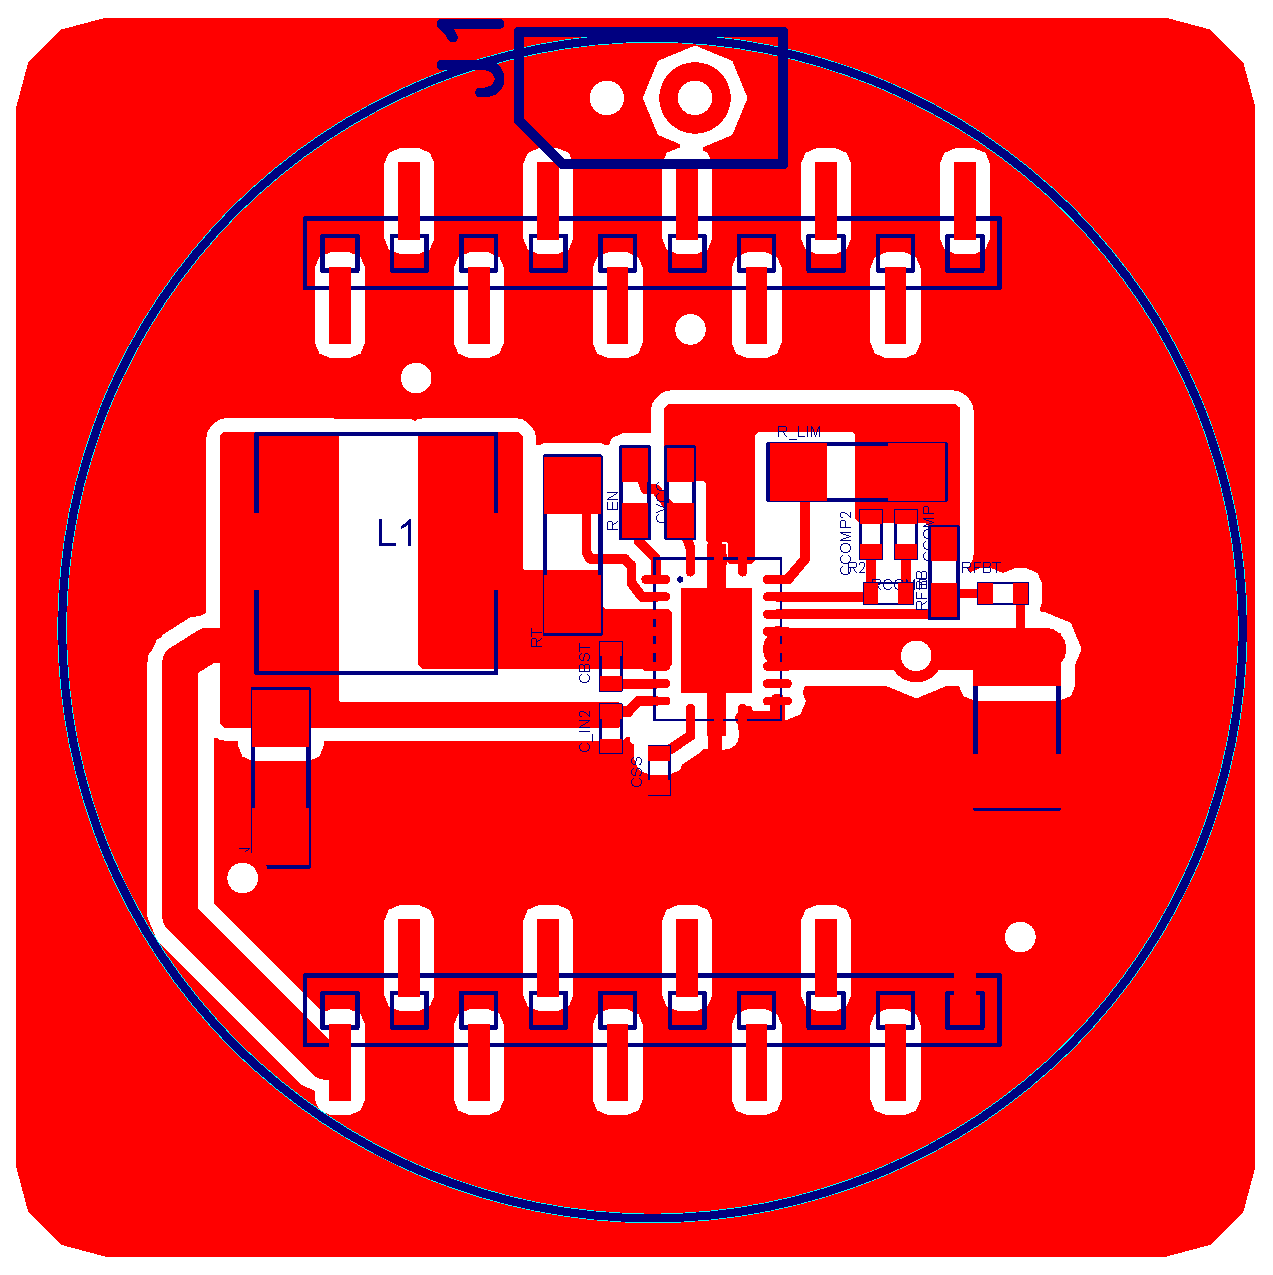
\includegraphics[width=2.0in]{./images/francis1}}\hfill
\subfigure[Back view]
  {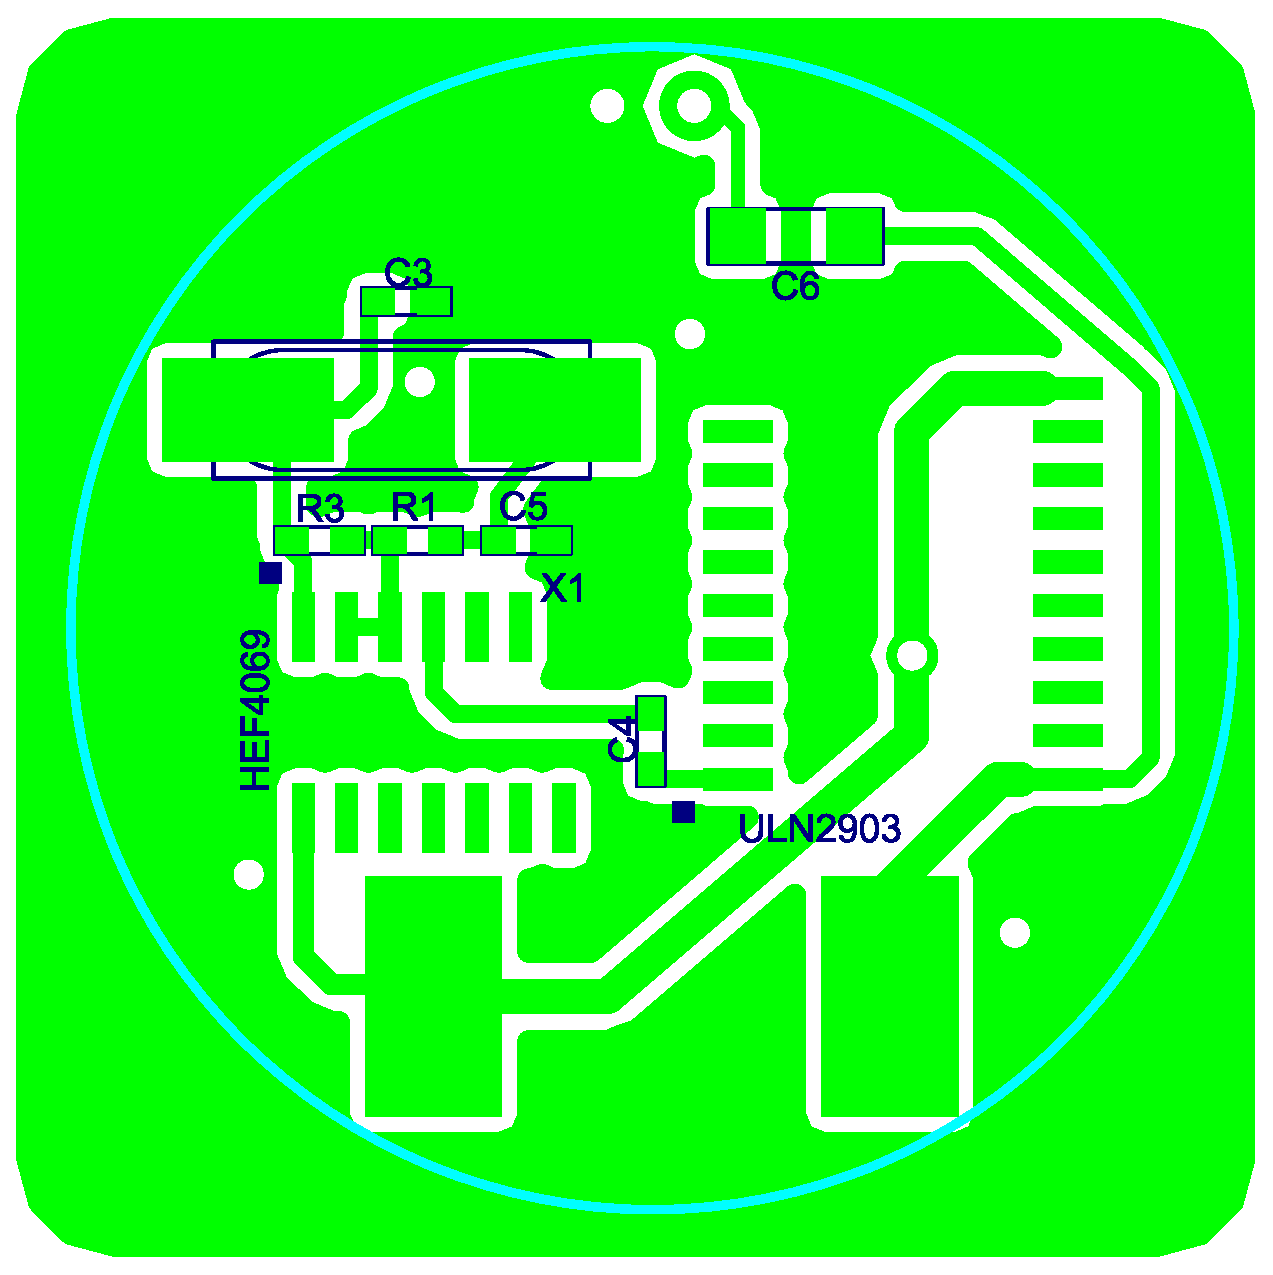
\includegraphics[width=2.0in]{./images/francis2}}
\hspace*{\fill}
\end{subfigmatrix}
\caption{Transmitter SMD design}
\end{figure}

Figure \ref{F:transmitter} exhibits the final transmitter board which is divided in two parts. The top side \ref{F:TX1} is composed by the power driver and the oscillator. It has the input coil pins to attach the primary inductor. The bottom side, invisible when the transmitter is connected to the \textit{Crazyflie}, is formed by the voltage regulator and the adapted pins. Those pins permit to connect directly the board to the quadcopter. The board height is small enough to avoid to graze the floor.


\begin{figure}[H]
\centering
\begin{subfigmatrix}{3}
\vspace{1em} 
\hspace*{\fill}%
\subfigure[Front view] 
  {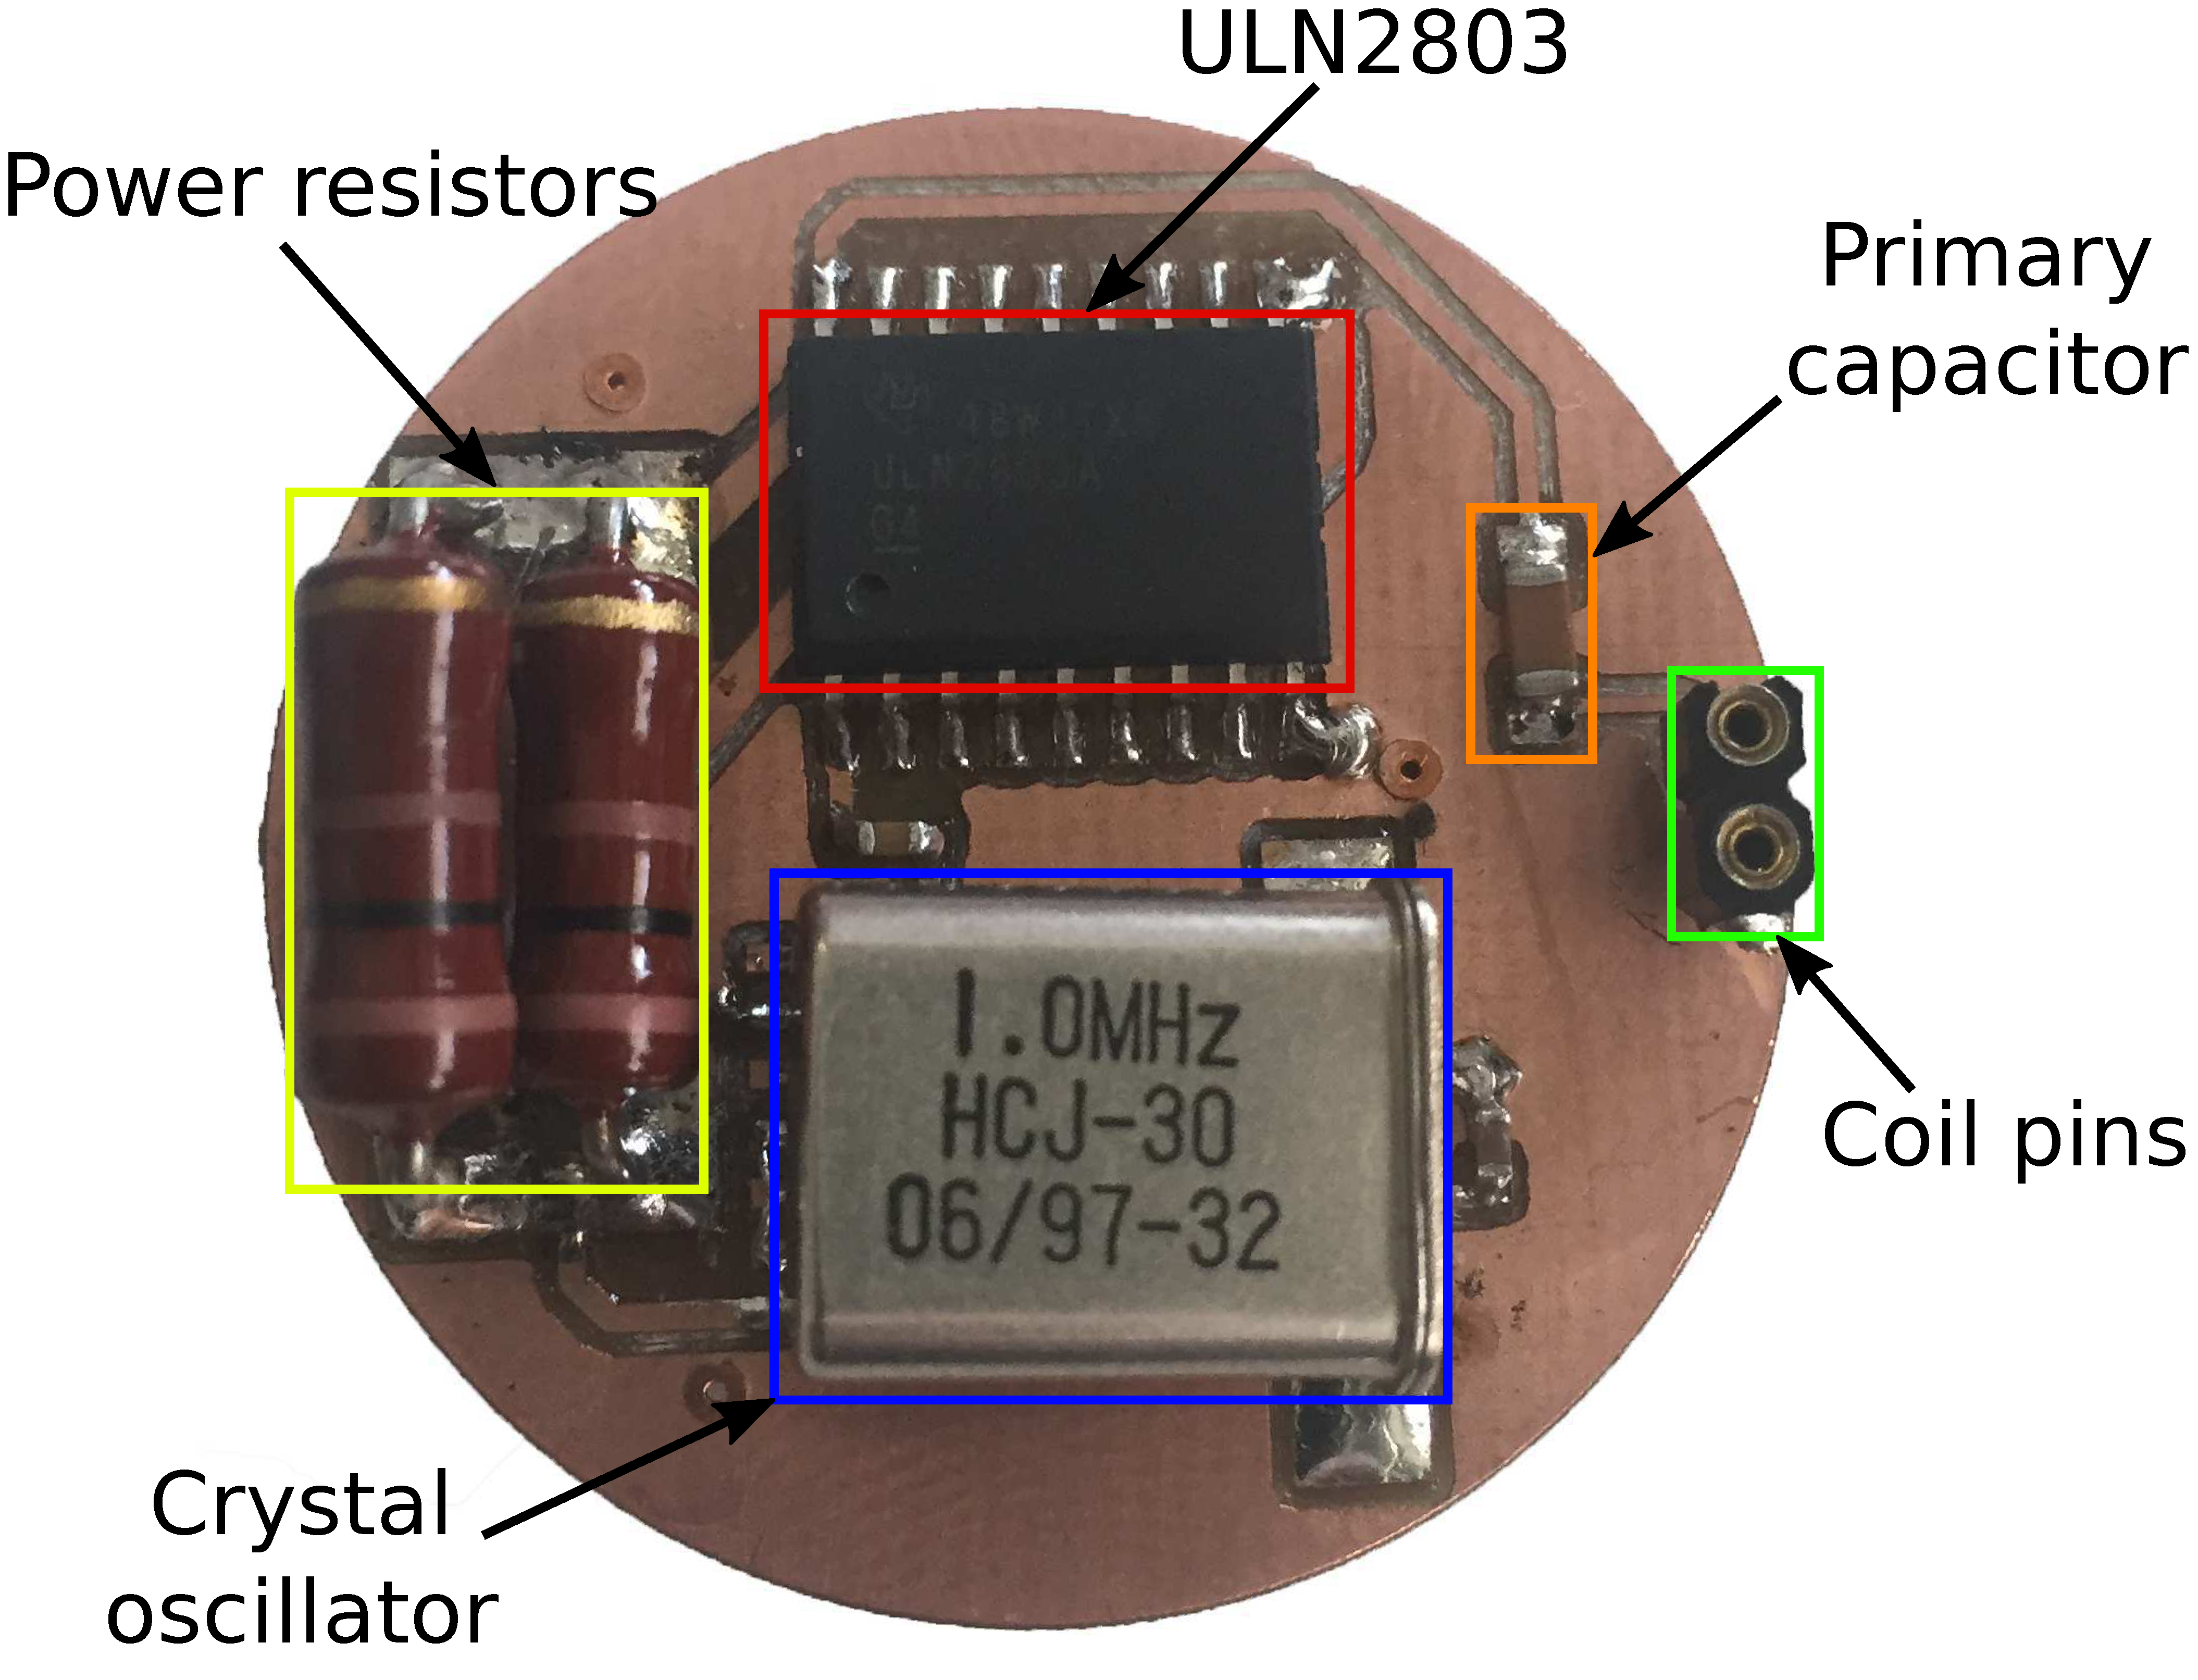
\includegraphics[width=2.0in]{./images/Transmitter_1X}\label{F:TX1}}\hfill
\subfigure[Side view] 
  {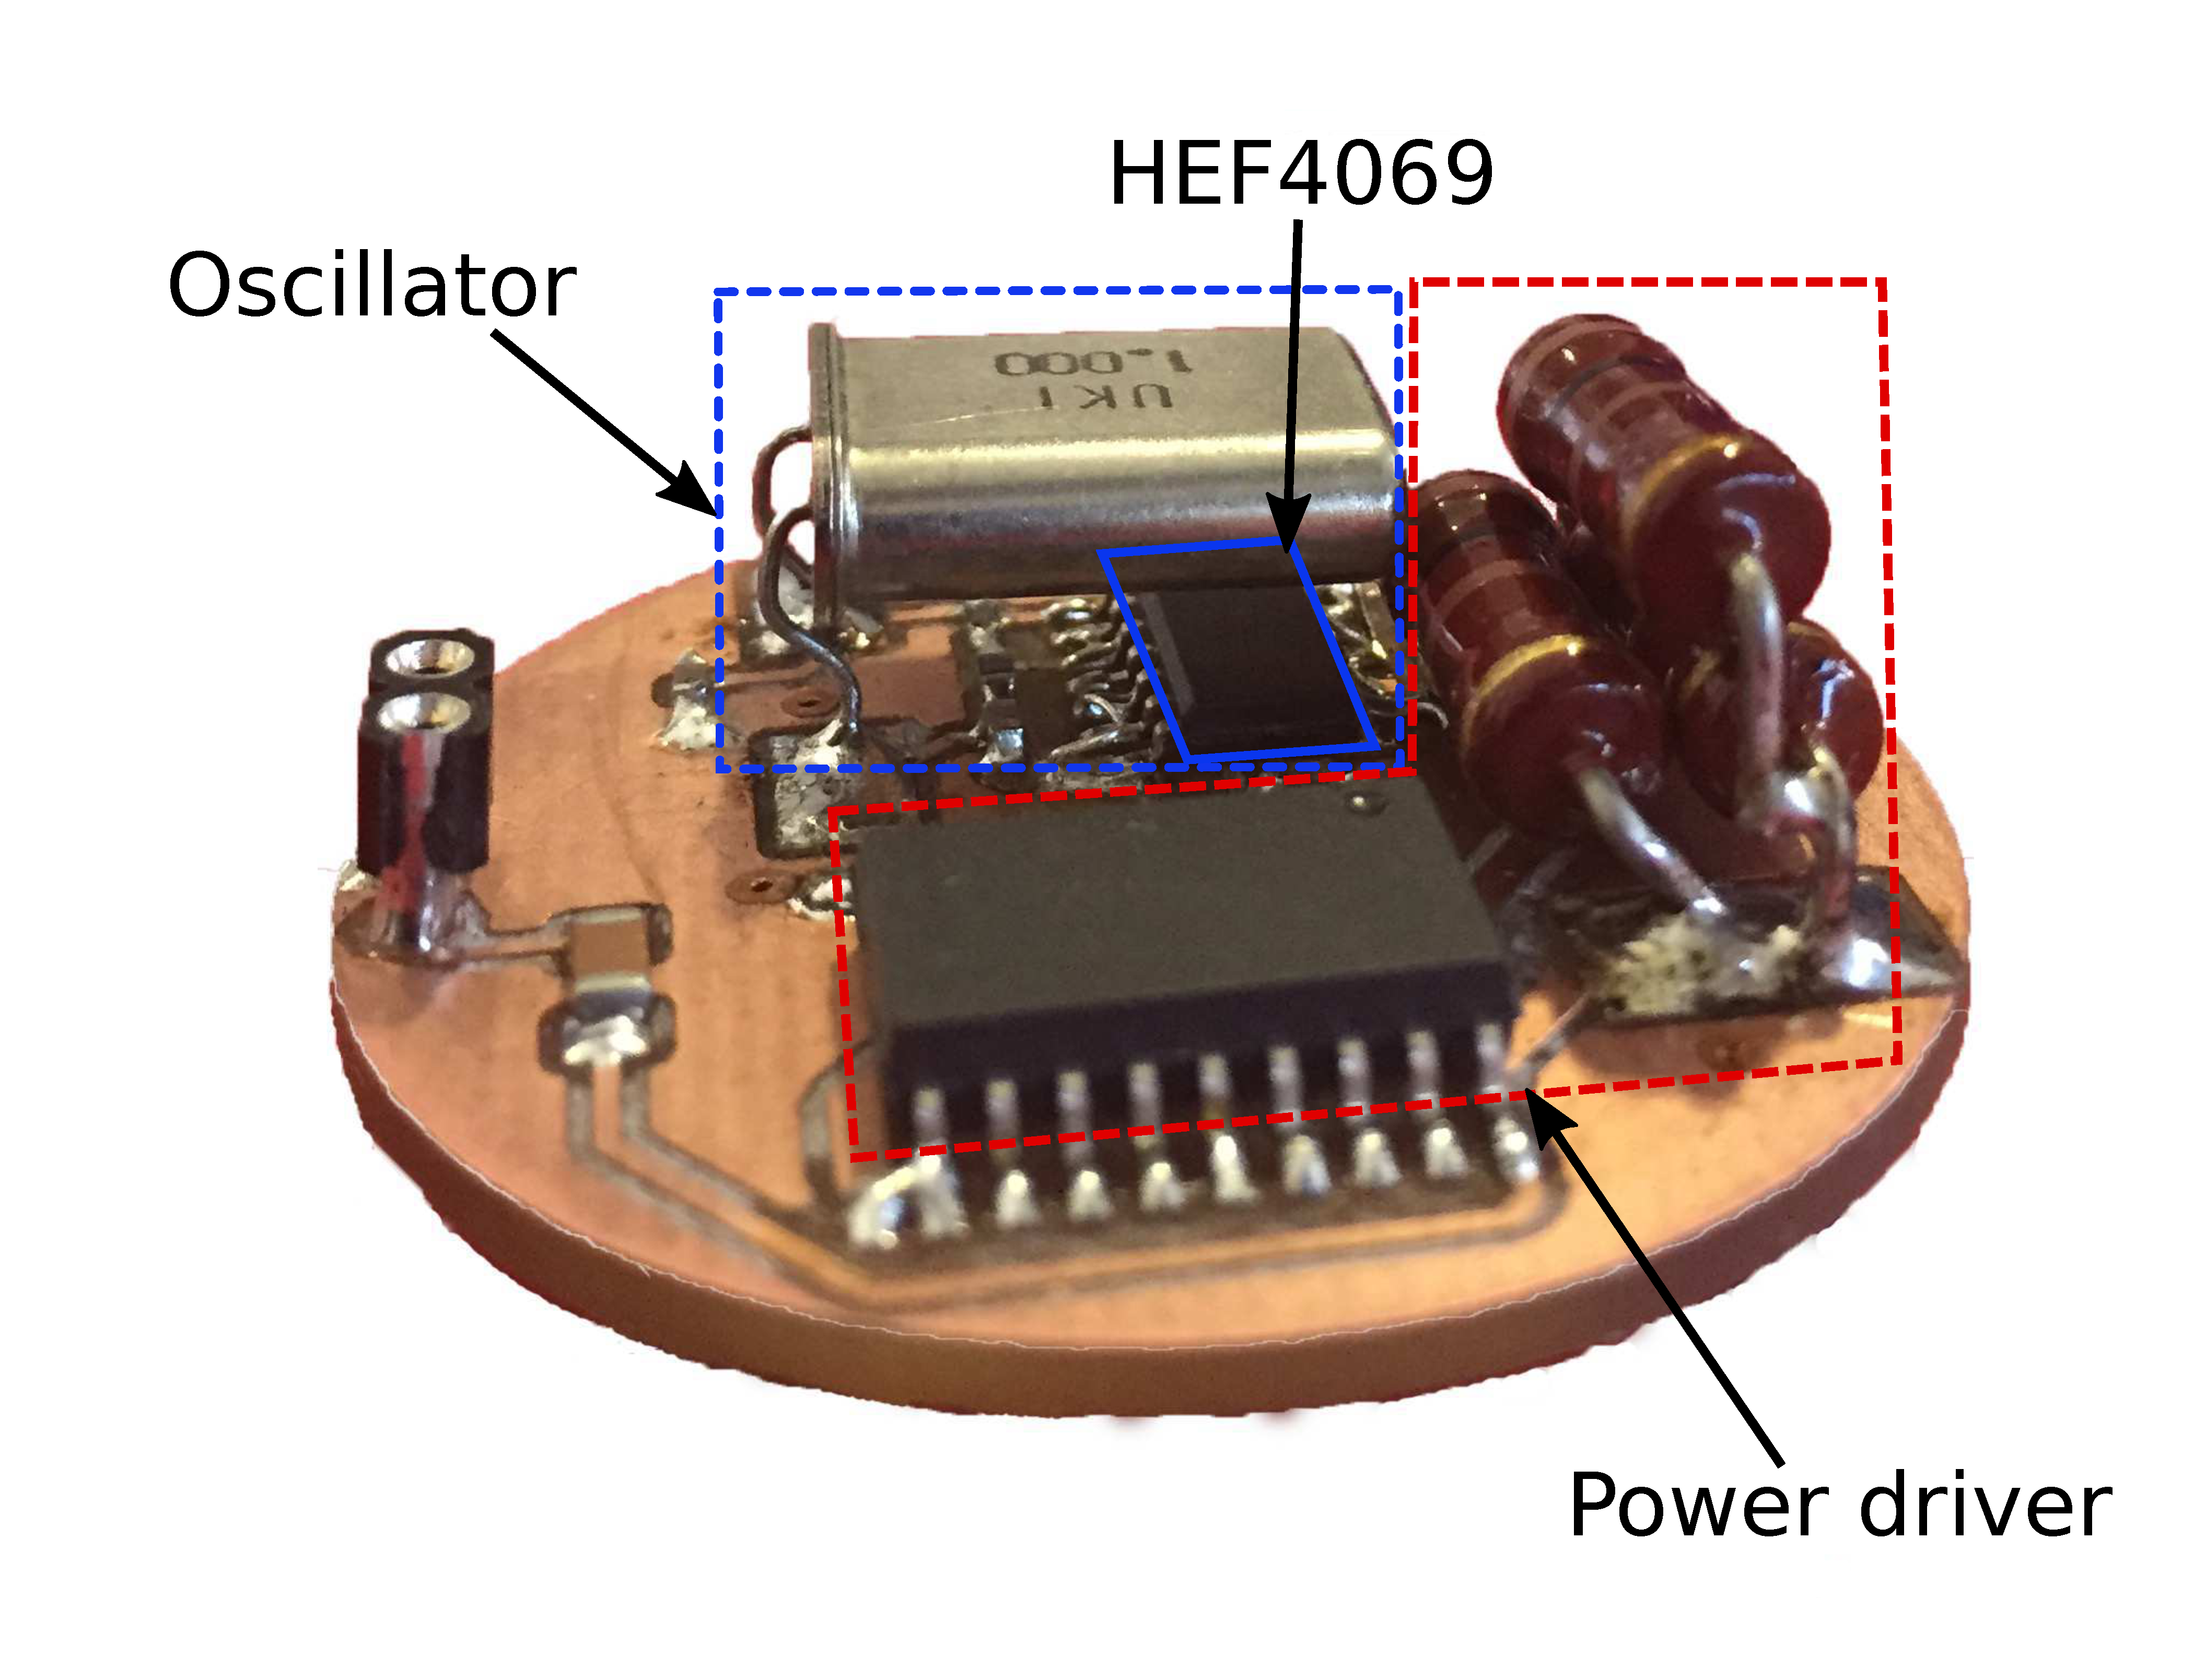
\includegraphics[width=2.0in]{./images/Transmitter_3}\label{F:TX3}}\hfill  
\subfigure[Back view]
  {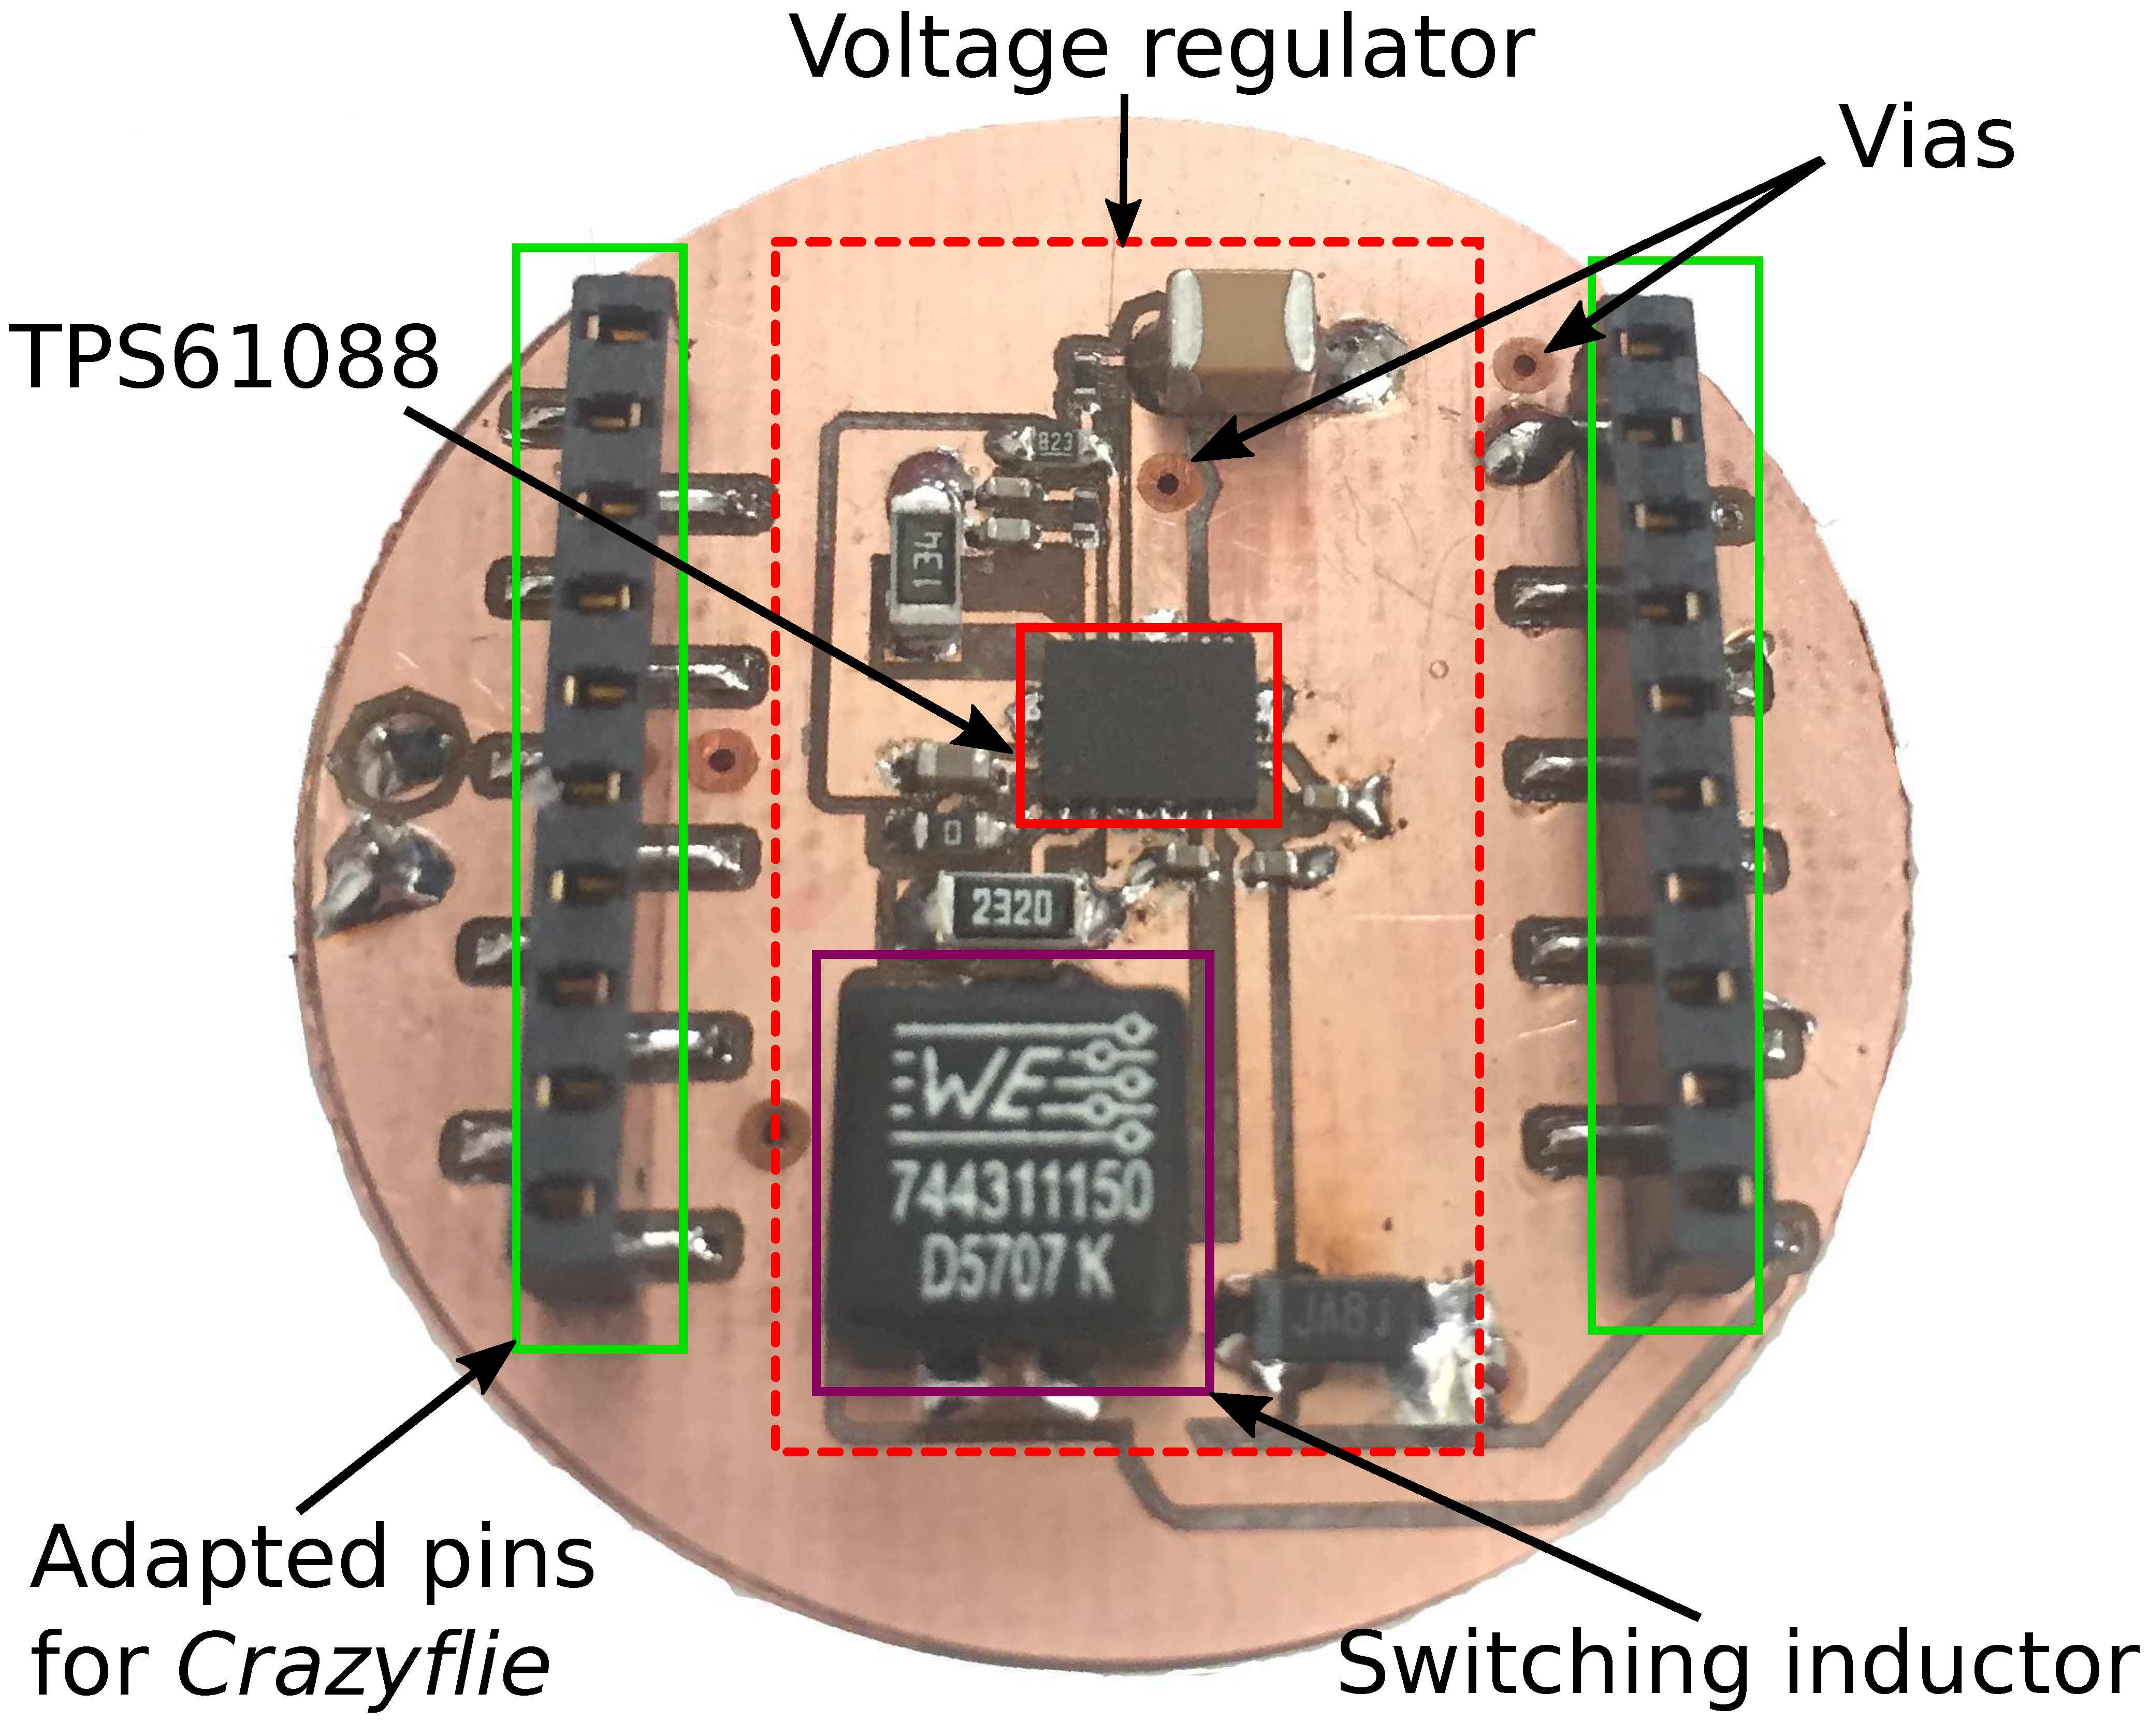
\includegraphics[width=1.9in]{./images/Transmitter_2Y}\label{F:TX2}}
\hspace*{\fill}%
\end{subfigmatrix}
\caption{Transmitter circuit}
\label{F:transmitter}
\end{figure}

Eventually, the total mass is computed using a precision scale. Table \ref{T:massConstraint} shows the mass of each section of the quadcopter. The experimental take-off mass depending on the motors thrust is shown in Figure \ref{F:thrust}. 

\begin{table}[htb]
\begin{center}
\begin{tabular}{|c|c|}

\noalign{\global\arrayrulewidth1pt}
\hline
\textbf{Element}  &   \textbf{Weight}\\
\hline
\hline
Battery             & 7.1 g     \\ \hline 
\textit{Tx} Coil    & 13.5 g    \\ \hline
\textit{Tx} Circuit & 8.5 g        \\ \hline
Crazyflie           & 8.3 g        \\ \hline
DC motors           & 4 x 2.8 g    \\ \hline
Motor mounts        & 4 x 0.8 g       \\ \hline
\hline
\textit{TOTAL}        & 51.8 g       \\ \hline

\end{tabular}
\caption{Mass constraint at transmitter side}
\label{T:massConstraint}
\end{center}
\end{table}


\begin{figure}[H]
  \begin{center} 
  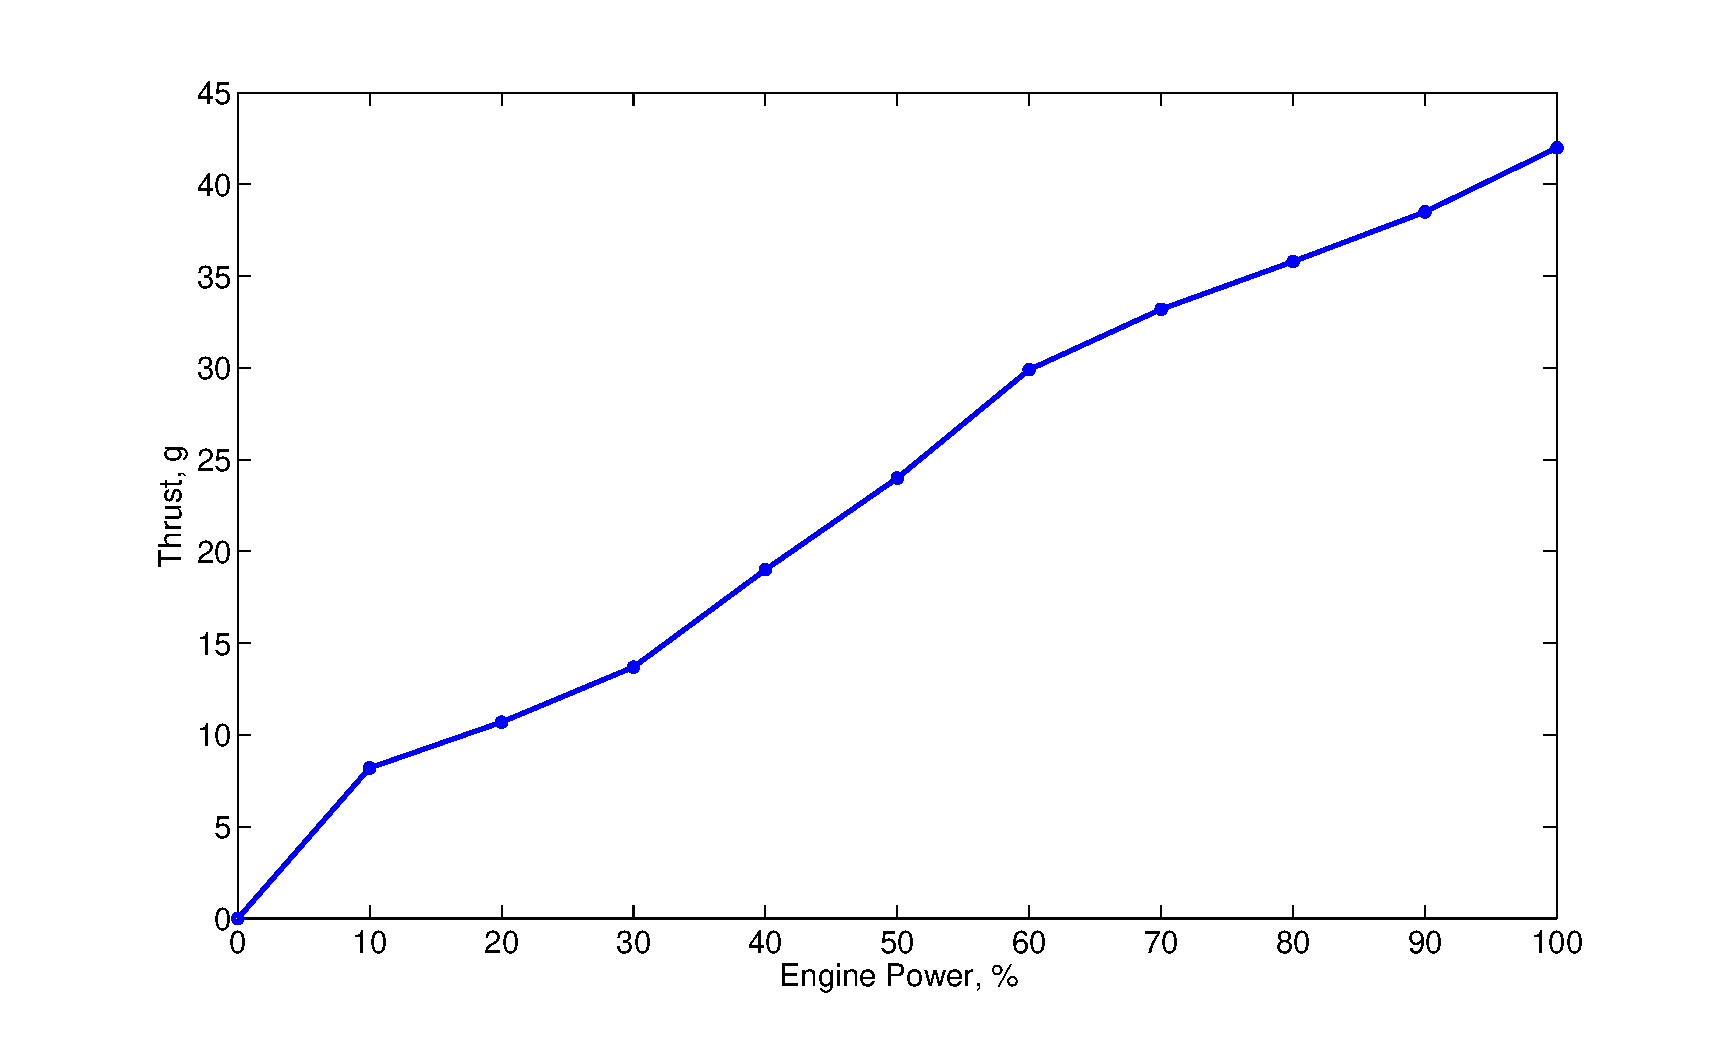
\includegraphics[width=0.9\textwidth]{./images/thrust}
    \caption{Thrust depending on the power level of the motors}
    \label{F:thrust}
  \end{center}
\end{figure}

\section{Receiver system}

The receiver side for a WPT system has the aim to rectify the transferred AC signal and, once it is in DC, to set it up to the desirable voltage levels. Depending on the application these two characteristic can be done in one stage. In the following sections the used circuits are explained in detail to accomplish a good signal rectification and conditioning. The chosen application for this project is presented is Section \ref{subsec:app}.

\subsection{Voltage Doubler}

To rectify the signal is selected a common used circuit for energy harvesting applications, the voltage doubler. This circuit is the perfect option for an energy harvesting. Owing to the low RF voltage levels, the doubler can rectify and condition at the same time. Voltage doubler circuits can be viewed as single stage or of a higher order multiplier; cascading identical stages together it is achieved a greater voltage multiplication. In Figure \ref{F:voltageDoubler} is shown a single stage for voltage doubler. 

\begin{figure}[ht!]
\begin{center}
\begin{circuitikz}
\ctikzset{v/.append style={/tikz/american voltages}}
\ctikzset{bipoles/resistor/height=0.25}
\ctikzset{bipoles/resistor/width=0.5}
\draw (0,2)
to[C=$C_1$] (2,2);
\draw (0,0)
to[short] (2,0)
to[D*] (2,2);
\draw (2,2)
to[D*] (4,2)
to[C=$C_2$] (4,0)
to[short] (2,0);
\draw (4,2)
to[short] (6,2);
\draw (4,0)
to[short] (6,0);
\node [ocirc] at (0,2) {$\qquad$};
\node [ocirc] at (0,0) {$\qquad$};
\node [ocirc] at (6,2) {$\qquad$};
\node [ocirc] at (6,0) {$\qquad$};
\node at (0,1) {$V_{in}$};
\node at (6,1) {$V_{out}$};
\node at (3,2.78) {$D_2$};
\node at (1.3,1) {$D_1$};
\end{circuitikz}
\caption{SIngle voltage doubler stage}
\label{F:voltageDoubler}
\end{center}
\end{figure}

An understanding of this circuit can be gained by interpreting firstly what occurs when the down swing of the AC current flows through the circuit. The diode $D_2$ blocks the current flow through $C_2$, but not the flow that goes across $C_1$. This current flow charges $C_1$ up to the same level of the AC voltage amplitude. Once the up swing of the AC voltage is reached, the voltage of both AC source and $C_1$ drop across $C_2$, charging it approximately twice the peak voltage of the AC signal \cite{doubler}.

As it is said in the first paragraph the voltage doubler is used in many energy harvesting applications, where the frequency goes from MHz to GHz. Thus, not all diodes are able to commute at these frequencies. The operating frequency of the inductive system of this project is set of 1 MHz and the selected diodes for assembling the voltage doubler are the HSMS-2850 Schottky diodes (SOT-23 Package) from \textit{Avago Technologies}:

\begin{figure}[htb]
\begin{center}
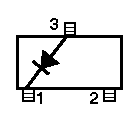
\includegraphics[width=0.2\textwidth]{./images/schottky}
\caption{SOT-23 Package for HSMS-2850 Schottky diode}
\end{center}
\end{figure}
The impedance of the HSMS-2850 diode can be linearly modeled as Figure \ref{F:schottky} shows \cite{doubler2}:

\begin{figure}[ht!]
\begin{center}
\begin{circuitikz}
\ctikzset{v/.append style={/tikz/american voltages}}
\ctikzset{bipoles/resistor/height=0.25}
\ctikzset{bipoles/resistor/width=0.5}
\draw (0,2)
to[R=$R_S$] (2,2)
to[vR=$R_j$] (4,2)
to[short] (8,2);
\draw (2,2)
to[short] (2,0)
to[C=$C_j$] (6,0)
to[short] (6,2);
\node [ocirc] (1) at (0,2) { };
\node [ocirc] (1) at (8,2) { };
\end{circuitikz}
\caption{Single voltage doubler stage}
\label{F:schottky}
\end{center}
\end{figure}

In this case $R_s$ and $C_j$ are the series resistance and the junction capacitance respectively, and $R_j$ has the following expression:

\begin{equation}
R_j = \frac{8.33\cdot{10^{-5}}\:n\:T}{I_b+I_s}
\end{equation}

where $n$ is the ideality factor, $T$ is the temperature in Kelvin degrees, $I_b$ is the externally applied bias current in amperes and $I_s$ is the saturation current. All this values, called \textit{SPICE}\footnote{\textit{SPICE} (Simulation Program with Integrated Circuit Emphasis) is a general-purpose, open source analog electronic circuit simulator.} parameters, are tabulated in Table \ref{T:SPICEparameters}.


\begin{table}[htb]
\begin{center}
\begin{tabular}{|c|c|c|}

\noalign{\global\arrayrulewidth1pt}
\hline
\textbf{Parameter}  &   \textbf{Units}  &   \textbf{HSMS-2850}\\
\hline
\hline
$C_j$            & pF  & $0.18$            \\ \hline 
$I_b$       & A &   $3\cdot{10^{-4}}$           \\ \hline 
$I_s$       & A &   $3\cdot{10^{-4}}$          \\ \hline 
$R_s$         & $\Omega $ &   $25$      \\ \hline
$n$         & $-$ &   $1.06$      \\ \hline
\end{tabular}
\caption{SPICE parameters for HSMS-2850}
\label{T:SPICEparameters}
\end{center}
\end{table}


The total impedance $Z_{diode}$ is given by:

\begin{equation}
Z_{diode} = R_S+\frac{R_j}{1+j\omega{C_j}R_j}
\end{equation}

In this project are used three stages for the design of the voltage doubler. This stages allows us to obtain good voltage levels at the output with good efficiency. Since, the more voltage doubler stages, the less efficiency.


\subsection{DC-DC boost converter}

The final stage introduced in the whole system is the \textit{bq25504 EVM}. As it is defined in its datasheet on the Appendices, the \textit{bq25504 EVM} is a ultra low power boost converter with battery management for energy harvester applications. This device is an evaluation module (EVM) programmed for deliver a 3.1 VDC maximum voltage (Over Voltage) for charging the storage element with a capacity larger than 100 $\mu$F. The supercapacitor or the battery allows the system to provide any peak currents that never would be obtained from the input source. 


The selection of the evaluation module is due to low power levels (among microwatts) needed to start converting the voltage to the programmed levels. The boost converter can be started with an input voltage lower than 330 mV. Below this level until 100 mV, it can operate but with more difficult. Once the 330 mV are reached, the boost converter will operate normally. This fact is called \textit{cold start}.

The following figure shows the schematic of the \textit{bq25504 EVM} and the output pins where the load and battery has to be placed:

\begin{figure}[H]
\begin{center}
\includegraphics[width=0.8\textwidth]{./images/bq25504}
\caption{\textit{bq25504 EVM} schematic}
\end{center}
\end{figure}


\subsection{Storage element}

Included as a part of the \textit{bq25504 EVM}, the storage element has to be analyzed in detail because, depending on the used application and power source there are different options to select. The first constraint is based on the ability of the power source to provide enough voltage during a period of time to charge high capacity batteries or capacitors. In this project, the nano-quadcopter performances do not allow to charge this kind of storage elements in a small period of time. Thus, the storage element selection is reduced to batteries or capacitors up to 500 mF of capacity. 

The total energy stored in a battery or capacitor is given by:

\begin{equation}
E = \frac{1}{2}\:C\:V^2
\end{equation}    

where $C$ is the capacitance of the storage element and $V$ is the stored voltage. Imagine that the system consume 1 A and the storage element has a capacitance of 1 F and is charged with 1 V; assuming the following equations and doing some calculus,

\begin{equation*}
t = \frac{E}{P}  
\end{equation*} 

\begin{equation*}
P = V\:I
\end{equation*}
 
the system will provide this current consumption during 0.5 seconds.

By the previous considerations, it is possible to select the storage element used to run the application. The chosen supercapacitor is selected from \textit{AVX BestCap}, and it has 140 mF of capacitance. This capacitance is adequate, taking into account the system performances. Its capacitance can provide peak currents of about milliamperes without any problem in a short period of time and still supplying voltage.

\subsection{Application} \label{subsec:app}

Eventually, the definition of the used application to demonstrate the capability of the designed inductive transfer system is explained in this section. In a first instance, the purpose was to implement a low consumption sensor as a load. Usually, these sensors have a high constant consumption that prevents the battery last enough time. To solve this problem, it is used the \textit{eZ430-RF2500}. This device is a wireless developing tool with an integrated temperature sensor. An \textit{eZ430-RF2500T} target board is connected in the receiver and communicates with the other target board installed on a USB debugging interface to show the air temperature using the Sensor Monitor Visualizer Application provided by the manufacturer. 

\begin{figure}[htb]
\begin{center}
\includegraphics[width=0.8\textwidth]{./images/RF5000}
\caption{\textit{eZ430-RF2500} debugging interface (left) and target board (right)}
\end{center}
\end{figure}

The main advantage is that the device consumption, when is in active mode, is about 270 $\mu$A typically. The only drawback is that \textit{eZ430-RF2500} needs 21.2 mA to communicate with the \textit{CC2500} radio-frequency transceiver. This peak current can be easily supplied by the selected supercapacitor, mentioned in previous section. The device specifications are exposed in its datasheet, given in the Appendices.


\subsection{Receiver Circuit Assembly}

As the receiver is not constrained in mass, the assembling of this part has been done in a \textit{stripboard}. Its relative small size allows to locate everywhere depending on the developed application. The resulting receiver circuit is exposed in Figure \ref{F:receiverC}.

\begin{figure}[H] 
\begin{center}
\includegraphics[width=0.6\textwidth]{./images/receiver222}
\caption{Receiver circuit}
\label{F:receiverC}
\end{center}
\end{figure}